\documentclass[a4paper]{article}
% !TeX spellcheck = en_GB

\usepackage{xspace}
\usepackage{graphicx}
\usepackage{wrapfig}
%\usepackage{doublespace}
\usepackage{setspace}
\usepackage{subcaption}
%\usepackage{boxedminipage}

% \newcommand{\QOSR}{QoS routing}
\newcommand{\ie}{i.e.,\xspace}
\newcommand{\eg}{e.g.,\xspace}
\newcommand{\cf}{c.f.,\xspace}

\newenvironment{problem}[1]%
{\noindent{}\textsc{Problem #1}: }{\vspace{12pt}}

\setlength{\hoffset}{0pt} \setlength{\voffset}{0pt}
\setlength{\oddsidemargin}{0pt} \setlength{\textwidth}{16cm}
\setlength{\topmargin}{-37pt} \setlength{\textheight}{670pt}
\setlength{\footskip}{60pt}

% \setstretch{2}

\begin{document}
\title{Shortest--path routing}
\author{Lars Staalhagen \\ Networks Technology and Service Platforms \\ DTU Fotonik Department of Photonics Engineering \\ larst@fotonik.dtu.dk}
\date{Version 2.0.1 --- \today}
\maketitle

\section{Introduction}
The purpose of this short lecture note is to introduce the concept of shortest path routing, which is an essential part of modern communication networks. The lecture note is primarily intended to be used in course 34355 Routing in Data Networks, and is loosely based on~\cite{ref:Bert} and~\cite{ref:Algo}.

\section{\label{sec:shortestpath}Shortest path routing}
The aim of shortest--path routing\footnote{In some textbooks, the term \emph{least--cost} routing is used instead.} is to find an optimal path in a network from a source node to a destination node. What constitutes an optimal path is decided by the network operator, i.e., it could be the path with the shortest end-to-end delay, the path with the highest capacity, or some other path.

The algorithms that are used to determine such an optimal path assume a graph--representation of the network, i.e., a graph, $G$ is a tuple, $G = (V,E)$, where $V$ is a set of the nodes in the graph and $E$ is a set of the edges\footnote{Other names are \emph{arcs} or \emph{lines}}. The nodes in the graph corresponds to routers in the real network, while the edges in the graph correspond to the communication links between routers. Since communication links can be either unidirectional (communication is only possible in one direction) or bi-directional (communication is possible in both directions), this must also be represented in the graph.
Figure~\ref{fig:Graph1c} shows a example of a graph with 5 nodes and 7 edges, where $V=\{A,B,C,D,E\}$ and
$E=\{(A,B),(B,A),(B,D),(C,A),(C,D),(D,C),(D,E),(E,B)\}$.
\begin{figure}[ht]
\centering
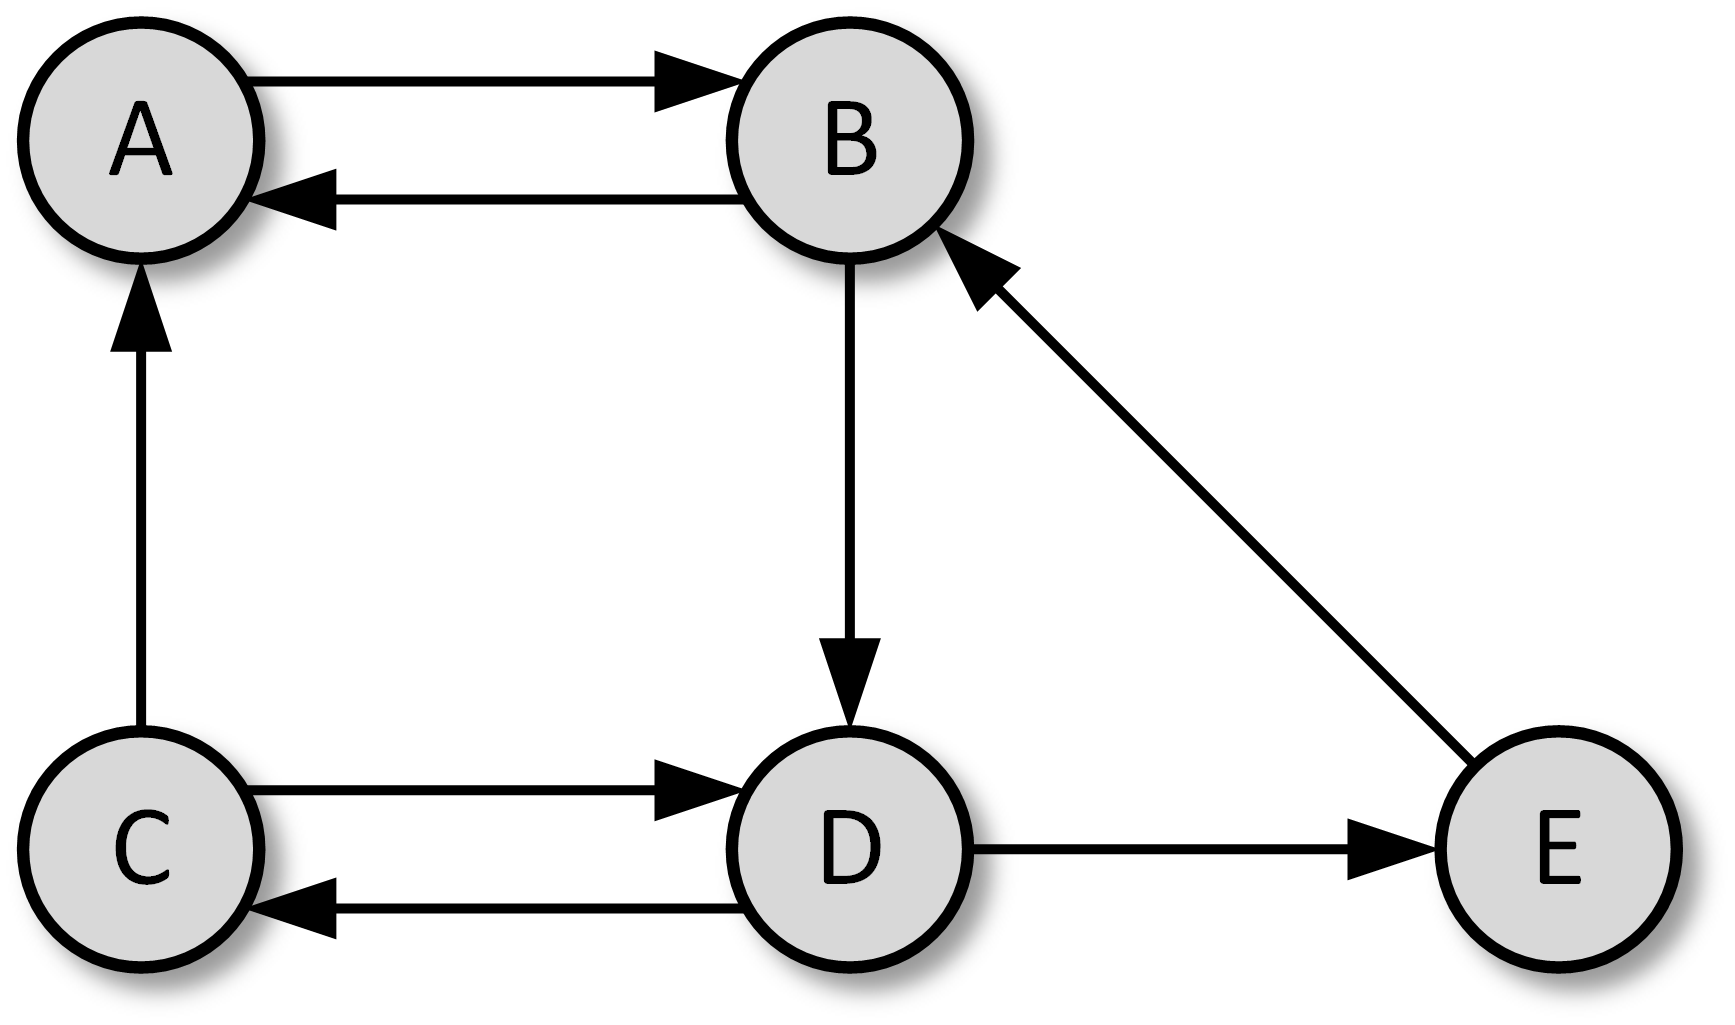
\includegraphics[scale=0.8]{graph1c.eps}
\caption{\label{fig:Graph1c}Sample graph.}
\end{figure}

In addition, a bi-directional link may be asymmetric in some sense, \ie the communication in the two directions may have different characteristics, \eg different delays. Therefore, the graph that is used to represent a network will be a \emph{weighted directed} graph. Every edge is associated with a metric (a number), which represent some characteristic of the link in the real network. If a physical link is bi-directional, and has the same metric in both directions, it is common to draw the edge as ''directionless'', \ie without an arrowhead, but it must be kept in mind, that this edge actually represents two directional edges. Part a of figure~\ref{fig:Graph1de} illustrates a weighted directed graph, while part b shows how the two edges between nodes C and D may be drawn as one.
\begin{figure}[ht]
\centering
\begin{subfigure}{.4\textwidth}
\scalebox{0.8}{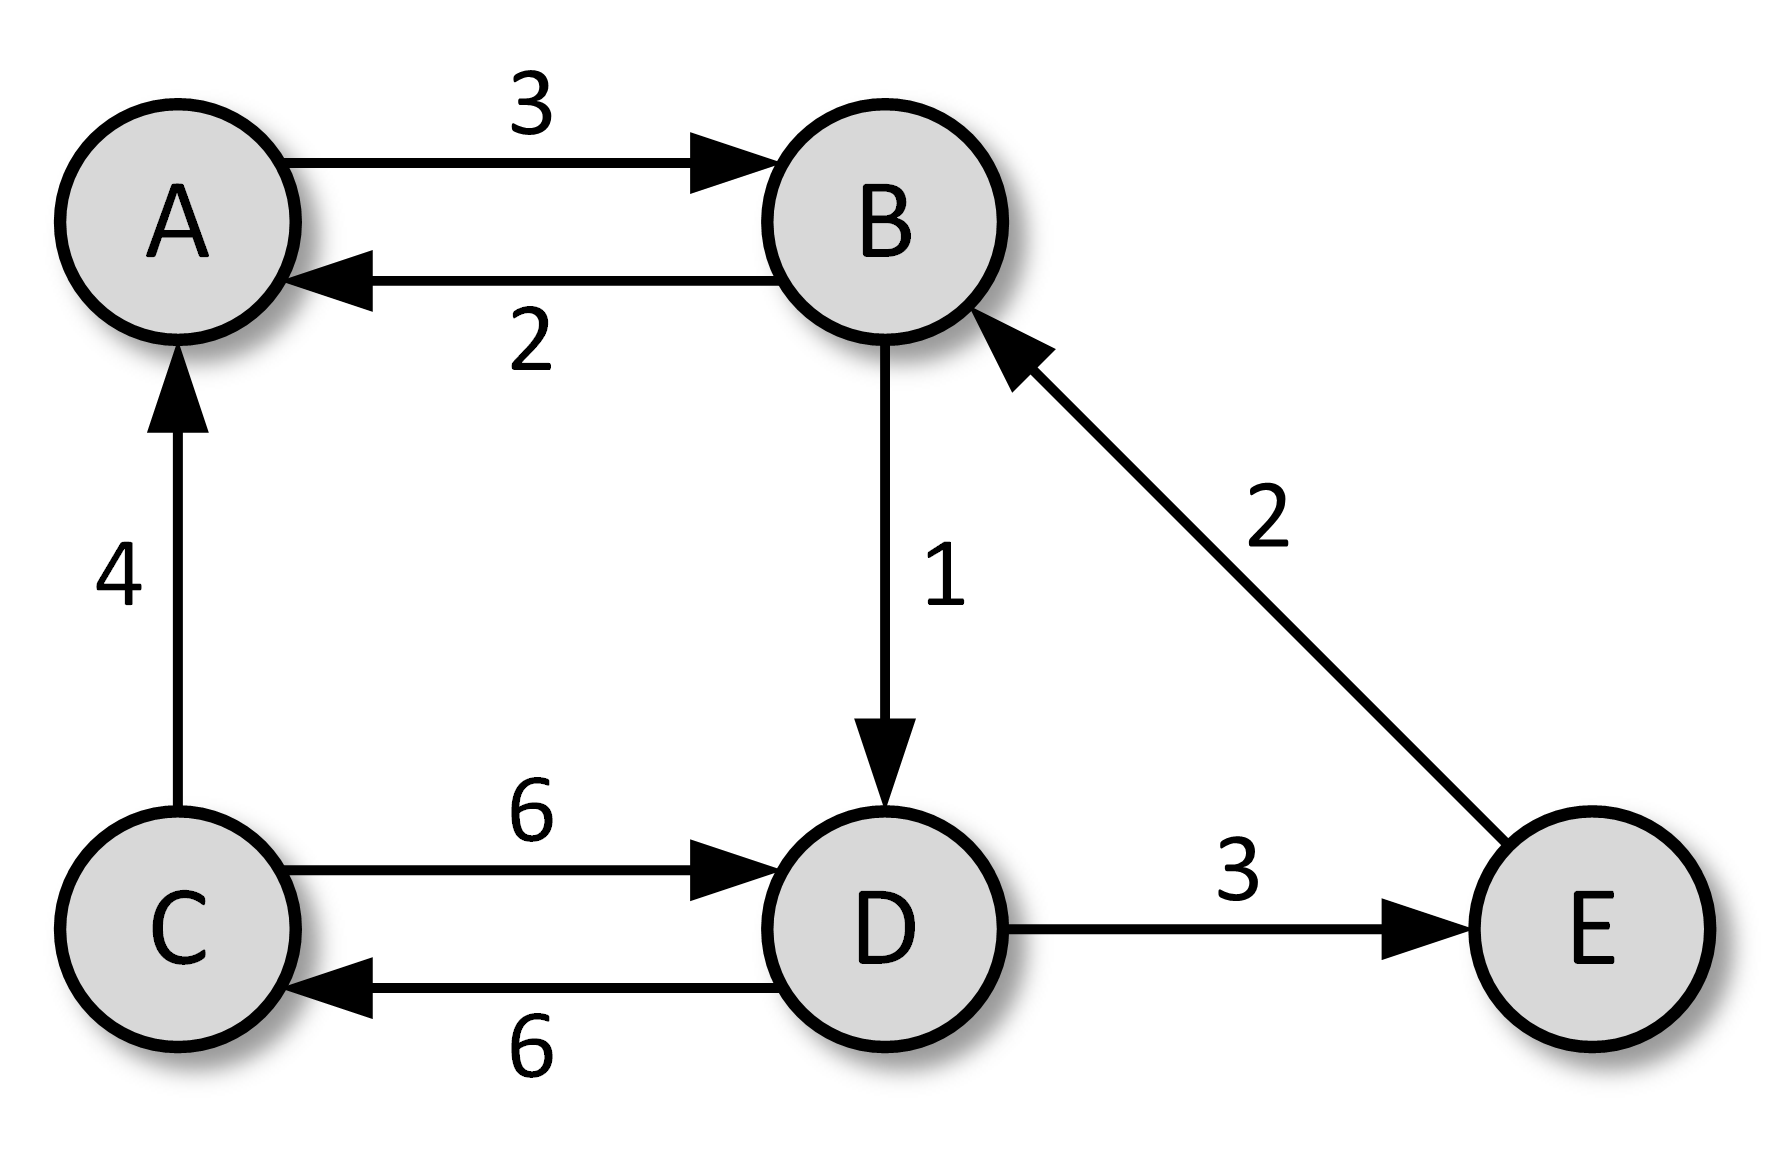
\includegraphics{graph1d.eps}}
\end{subfigure}
\hspace{1cm}
\begin{subfigure}{.4\textwidth}
\scalebox{0.8}{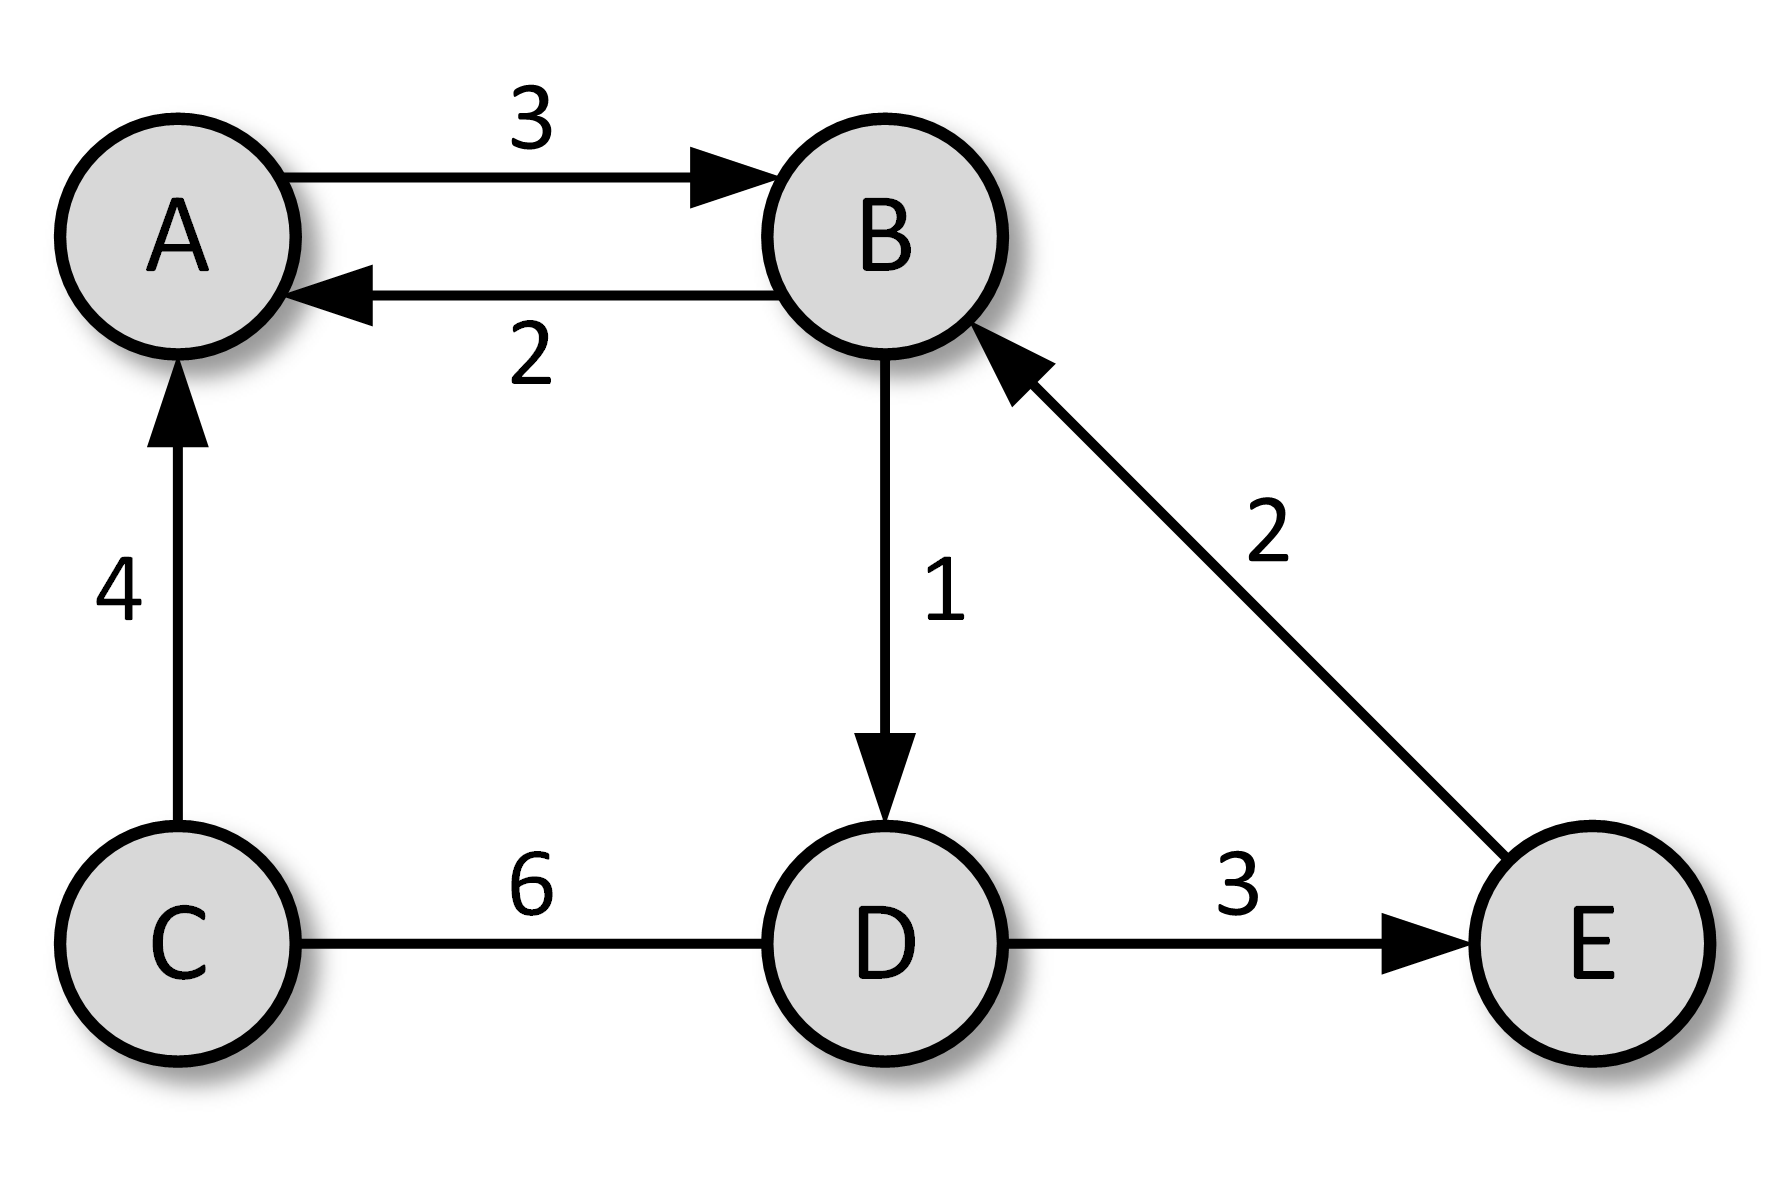
\includegraphics{graph1e.eps}}
\end{subfigure}
\caption{\label{fig:Graph1de}Collapsing edges with identical metrics into ''direction less'' edge (between nodes C and D).}
\end{figure}

The metrics that are associated with the edges in the graph can be thought of as the \emph{length} of that edge. Therefore, a path from one node to another in the graph has a total length of the sum of the length of the edges that are part of the path. In this sense, the metrics are \emph{additive}, that is, the total length of the path is the sum of the length of the different edges that are part of this path.

The purpose of shortest--path routing is then to find paths in the graph that minimizes the path--lengths. The simplest problem would be to find the shortest--path from a given source--node to a given destination--node, but the common algorithms today determine the shortest--paths from a given source node to \emph{all} other nodes in the graph. A number of algorithms exist that can be used to determine the shortest paths, but in connection with communication networks, the most common are the \emph{Bellman-Ford} algorithm and the \emph{Dijkstra} algorithm. The former is used in a distributed version in connection with the RIP routing protocol, while the latter is used with the OSPF protocol.

As described earlier, the metrics associated with the edges in the
graph correspond with some characteristic of the physical link in the
network. Examples of these metrics include:
\begin{itemize}
%
\item Delay -- the metric is (directly) proportional with the delay on the link, so that the shortest--path from the source to the destination is the path that minimizes the end--to--end delay. The link--delay may include any buffering delay at the sending node.
%
\item Economical cost -- the metric is (directly) proportional with the expenditure of transmitting information on the link. The shortest--path is then the path that minimizes the expenditure for the network operator.
%
\item Error rate -- the metric is a function of the link's error rate\footnote{Note that the metric and the link's error rate are not directly proportional in this case.}, so that a link with a high error--rate is depicted in the graph as an edge with a high cost. Finding the path in the graph that minimizes the sum of the edge metrics would then tend to favour links with lower error rates, since they would have a smaller metric.
%
\end{itemize}
In general, the link metrics may also be a function of (some of) the
parameters of a link, i.e.
\[
\textrm{Metric} = f(\textrm{delay}, \textrm{economical cost}, \ldots)
\]

In mathematical terms, the link--metrics are here denoted by $C_{ij}$
for the metric on the link \emph{from} node $i$ \emph{to} node $j$. In
general, $C_{ij}\ne{}C_{ji}$, i.e. for a bi-directional link, the
metrics are generally different in the two directions, \eg if the
metrics are a function of the link delays. By definition,
$C_{ii}=0$, since (informally) the distance from node $i$ to node $i$
is of course 0. Furthermore, two different nodes, $i$ and $j$, might
not have a direct edge between them, so it is impossible to send a
packet directly from node $i$ to node $j$. This situation is
represented in the metrics as $C_{ij}=\infty$.

The results of the shortest--path calculations are stored in the
source--node's routing table. If the network uses
\emph{source--routing}, the entire paths are stored since they
must be included in the packets. If the network uses
\emph{hop--by--hop} routing, the source node will only need to
store the identity of the next--hop node for all destinations.

\subsection{Bellman-Ford algorithm}
The Bellman-Ford algorithm can be described as follows:

\begin{figure}[ht]
\setlength{\fboxsep}{9pt}
\begin{center}\noindent\fbox{\begin{minipage}[h]{0.9\textwidth}
\paragraph{Definitions:}
$s$ = Source node. $D^{h}_{j}$ = The cost of shortest path from $s$ to
node $j$ under the condition that the path contains at most $h$
links.
\vspace{9pt}
\paragraph{Initialization:}
$\forall h: D^{h}_s = 0$ and $\forall j\neq{}s:D^{0}_j =  \infty$.
\vspace{9pt}
\paragraph{Iteration:}
$\forall j : D^{h+1}_{j} = \min_{k}\left(D^{h}_k + C_{kj}\right).$
Keep repeating the iteration until $\forall j: D^{h+1}_j =
D^{h}_j$.
\end{minipage}}
\end{center}
\caption{\label{fig:BFAlgo}Bellman-Ford algorithm}
\end{figure}

\noindent{}Consider the graph in figure~\ref{fig:SP_Graph}.
\begin{figure}[ht]
\centering
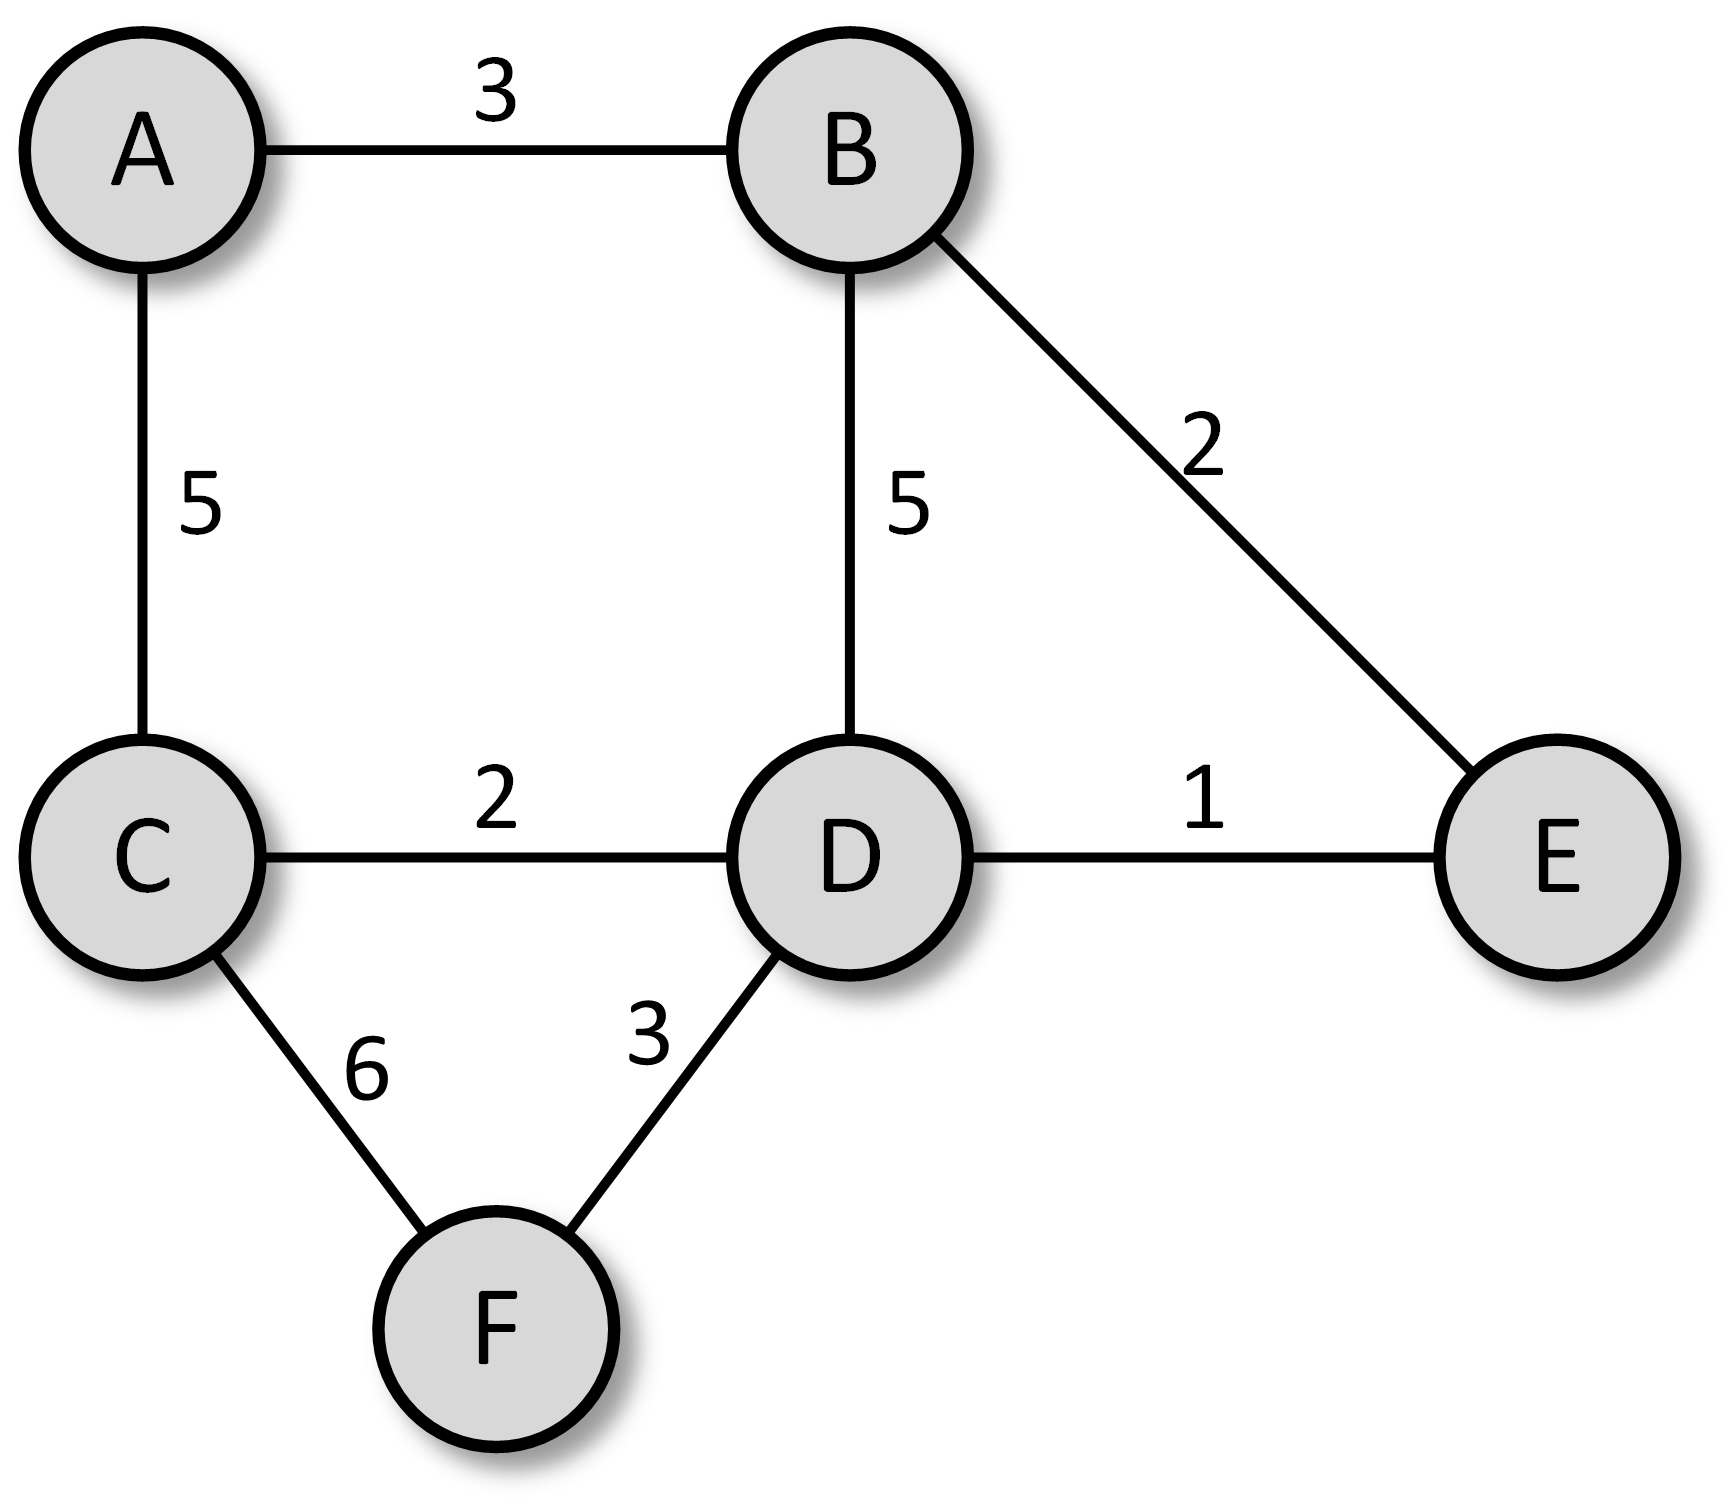
\includegraphics[scale=0.8]{sp_graph.eps}
\caption{\label{fig:SP_Graph}Example network.}
\end{figure}

\noindent{}If we want to calculate the shortest paths from node A
to all other node in this network, we get the results, shown in
table~\ref{tbl:BF-Results}.

\begin{table}[ht]
\centering
\begin{tabular}{|c|c|c|c|c|c|c|c|c|c|c|}\hline
%
 & \multicolumn{2}{|c|}{Node B} & \multicolumn{2}{|c|}{Node C} &
 \multicolumn{2}{|c|}{Node D} & \multicolumn{2}{|c|}{Node E} &
 \multicolumn{2}{|c|}{Node F}\\ \hline
%
$h$ & $D^{h}_B$ & Path & $D^{h}_C$ & Path & $D^{h}_D$ & Path &
$D^{h}_E$ & Path & $D^{h}_F$ & Path \\ \hline
%
0 (Init) & $\infty$ & --- & $\infty$ & --- & $\infty$ & --- &
$\infty$ & --- & $\infty$ & --- \\ \hline
%
1 & 3 & A--B & 5 & A--C & $\infty$ & --- & $\infty$ & --- &
$\infty$ & --- \\ \hline
%
2 & 3 & A--B & 5 & A--C & 7 & A--C--D & 5 & A--B--E & 11 & A--C--F \\
\hline
%
3 & 3 & A--B & 5 & A--C & 6 & A--B--E--D & 5 & A--B--E & 10 & A--C--D--F \\
\hline
%
4 & 3 & A--B & 5 & A--C & 6 & A--B--E--D & 5 & A--B--E & 9 &
A--B--E--D--F \\ \hline
%
5 & 3 & A--B & 3 & A--C & 6 & A--B--E--D & 5 & A--B--E & 9 &
A--B--E--D--F \\ \hline
\end{tabular}
\caption{\label{tbl:BF-Results}Bellman-Ford calculation of
shortest paths}
\end{table}

Since $D^{5}_{j} = D^{4}_{j}$ for all $j$, the algorithm has
converged, and the contents of the routing table for node A will
then be as shown in table~\ref{tbl:RoutingTbl-A}.
\begin{table}[ht]
\centering
\begin{tabular}{|c|c|c|}\hline
%
Destination & Path (source--routing) & Next--hop (hop--by--hop
routing) \\ \hline
%
B & A--B & B \\ \hline
%
C & A--C & C \\ \hline
%
D & A--B--E--D & B \\ \hline
%
E & A--B--E & B \\ \hline
%
F & A--B--E--D--F & B \\ \hline
\end{tabular}
\caption{\label{tbl:RoutingTbl-A}Contents of routing table for
node A.}
\end{table}

At this point, the shortest--paths from the source node to all
other nodes in the network have been found, but in general, we
need the shortest--paths between any pair of nodes in the network.
For this, it is necessary to execute the Bellman-Ford algorithm
$V$ times, using (in turn) every node in the network as the
source node in the algorithm.

\subsection{Distributed Bellman-Ford}
\noindent{}The Bellman-Ford algorithm can also be implemented in
a distributed version. To implement this, a node must from time to
time transmit information from its entire routing table to all its
neighbour\footnote{Two nodes are considered neighbours, if they can
  communicate directly, \ie that there is a link between the two
  nodes} nodes. It can be shown that as long as all nodes from time to
time transmit this information, the optimal shortest--paths will be
determined eventually.

The idea behind the distributed Bellman-Ford is that, whenever a
node receives information from a neighbour node, it will determine
whether the information will lead to a better (smaller cost) path
than previously known. As an example, consider
figure~\ref{fig:Dist_BF_Ex}: Suppose that node A receives the
following information from node B: ''I can reach node Z with a cost
of $\alpha$'' and from C: ''I can reach node Z with a cost of
$\beta$''. Node A would then determine, which of these possible
ways of reaching node Z would be better by determining the minimum
of $C_{AB} + \alpha$ and $C_{AC} + \beta$. If $C_{AB} + \alpha <
C_{AC} + \beta$ then the (currently) best path from A to Z is via
node B; otherwise it is via node C.

\begin{figure}[!ht]
\centering
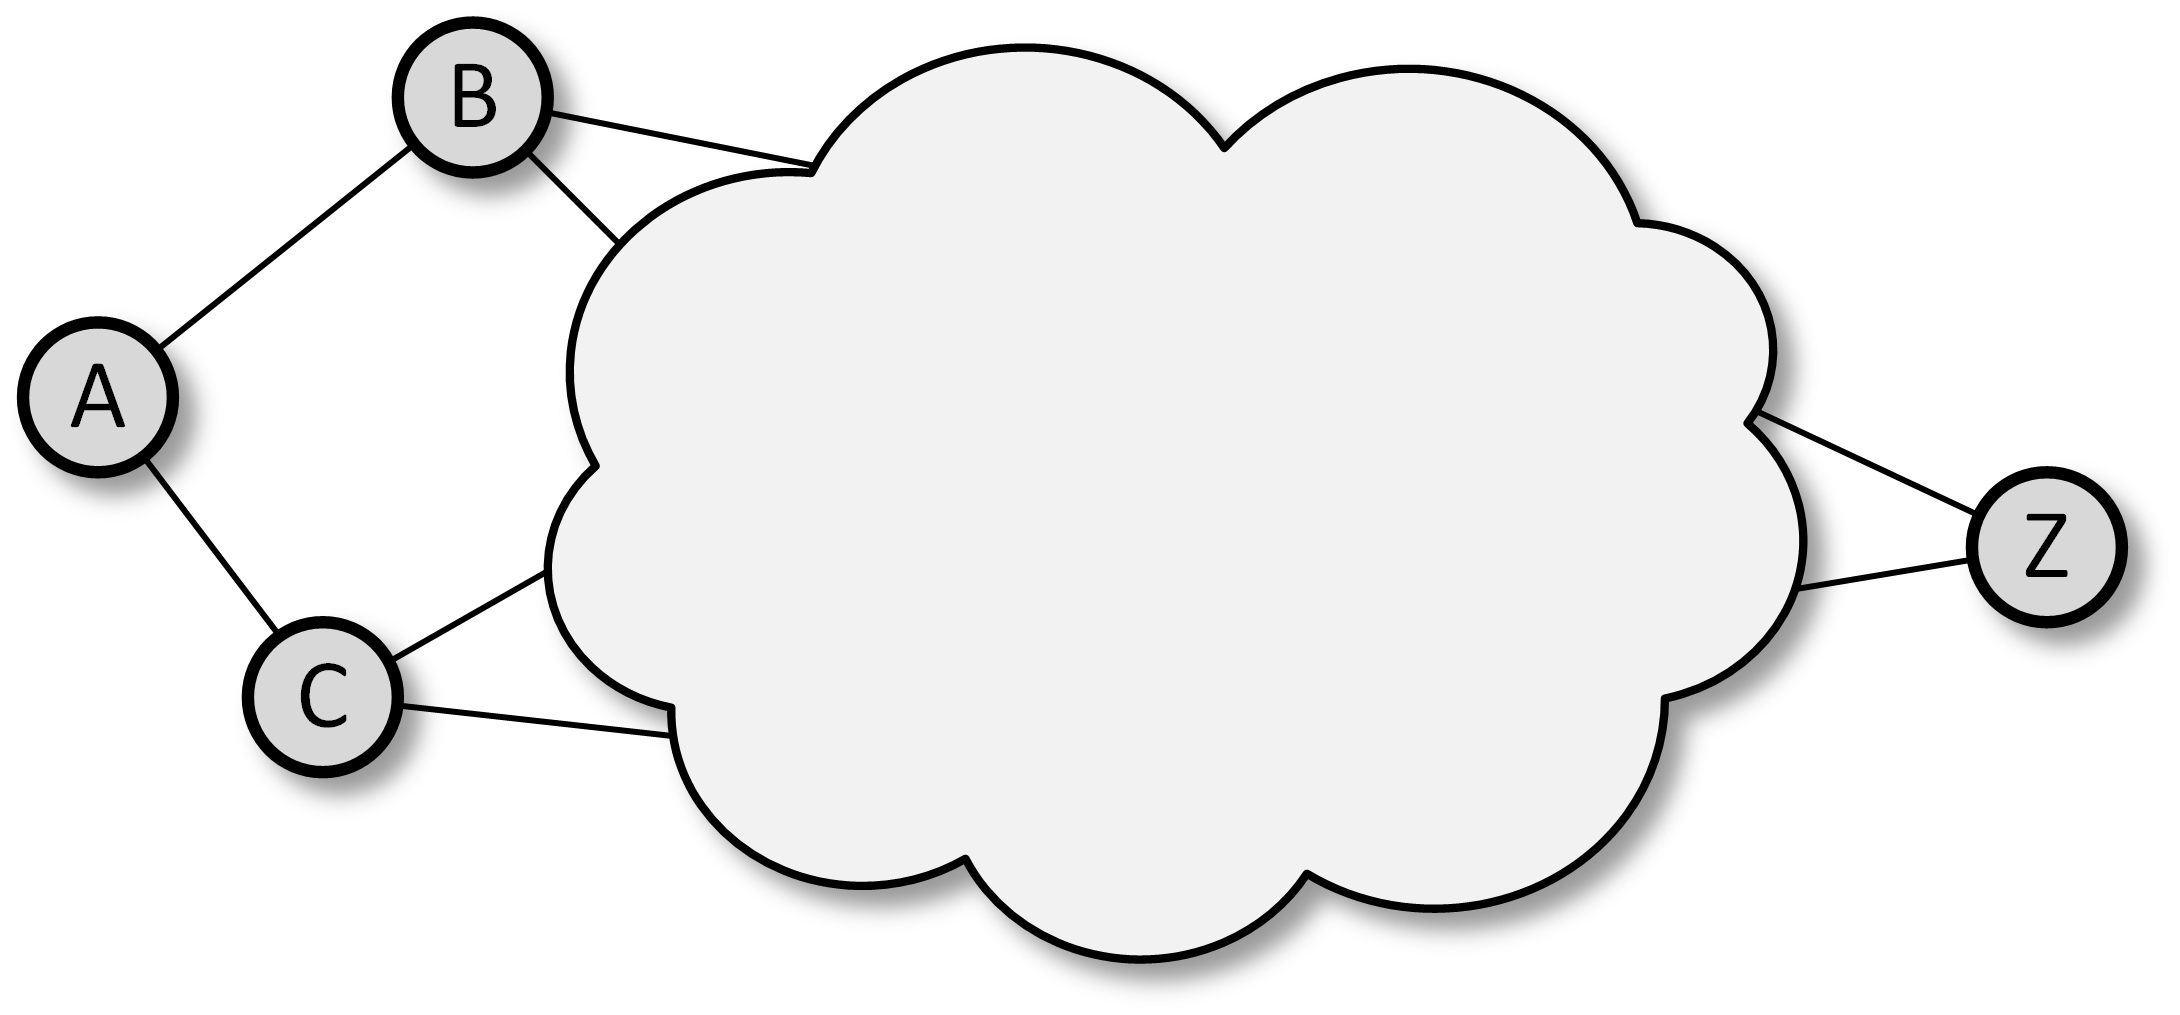
\includegraphics{dist_bf_ex.eps}
\caption{\label{fig:Dist_BF_Ex}Example network for the distributed
Bellman-Ford.}
\end{figure}

This description of the distributed version of the Bellman-Ford
algorithm is very simplified. The RIP routing protocol uses the
distributed Bellman-Ford algorithm, but with a number of additional
facilities.

\subsection{Dijktra's algorithm}
Dijkstra's algorithm can be described as shown in
figure~\ref{fig:DAlgo}.

\begin{figure}[ht]
\setlength{\fboxsep}{9pt}
\begin{center}\noindent\fbox{\begin{minipage}[h]{0.9\textwidth}
\paragraph{Definitions:}
$s$ = source node. $D_j$ = (estimate) of the cost of the shortest
path from $s$ to (destination) node $j$. $M$ = set of nodes.
\vspace{9pt}
\paragraph{Step 1:}
Initialize the set $M$ with just the source node, $M=\{s\}$.
\vspace{9pt}
\paragraph{Step 2:}
Find the node with the smallest $D_j$ that is not yet included in
the set $M$ and add this node to $M$: $D_k = \min_{j\not\in M}
D_j$. $M \gets M \cup \{k\}$. \vspace{9pt}
\paragraph{Step 3:}
For all nodes not (yet) included in $M$, check if a path through
the just--added node (node $k$) would be better than the current
path: $D_j = \min(D_j, D_k + C_{kj})$. \vspace{9pt}
\paragraph{Step 4:}
If $V\neq{}M$ continue from step 2; otherwise the algorithm has
terminated.
\end{minipage}}
\end{center}
\caption{\label{fig:DAlgo}Dijkstra's algorithm}
\end{figure}

\noindent{}If we use Dijkstra's algorithm on the network in
figure~\ref{fig:SP_Graph}, we get table~\ref{tbl:dijkstra}. The
routing table of node A will of course be the same as in the
Bellman-Ford example.

\begin{table}[ht]
\centering\begin{tabular}{|c|c|c|c|c|c|c|c|c|c|c|}\hline
 & \multicolumn{2}{|c|}{Node B} & \multicolumn{2}{|c|}{Node C} &
 \multicolumn{2}{|c|}{Node D} & \multicolumn{2}{|c|}{Node E} &
 \multicolumn{2}{|c|}{Node F}  \\ \hline
$M$ & $D_B$ & Path & $D_C$ & Path & $D_D$ & Path & $D_E$ & Path &
$D_F$ & Path \\ \hline
%
$\{A\}$ & 3 & A--B & 5 & A--C & $\infty$ & --- & $\infty$ & --- &
$\infty$ & --- \\ \hline
%
$\{A,B\}$ & 3 & A--B & 5 & A--C & 8 & A--B--D & 5 & A--B--E &
$\infty$ & --- \\ \hline
%
$\{A,B,C\}$ & 3 & A--B & 5 & A--C & 7 & A--C--D & 5 & A--B--E & 11
& A--C--F \\ \hline
%
$\{A,B,C,E\}$ & 3 & A--B & 5 & A--C & 6 & A--B--E--D & 5 & A--B--E
& 11 & A--C--F \\ \hline
%
$\{A,B,C,D,E\}$ & 3 & A--B & 5 & A--C & 6 & A--B--E--D & 5 &
A--B--E & 9 & A--B--E--D--F \\ \hline
%
$\{A,B,C,D,E,F\}$ & 3 & A--B & 5 & A--C & 6 & A--B--E--D & 5 &
A--B--E & 9 & A--B--E--D--F \\ \hline
\end{tabular}
\caption{\label{tbl:dijkstra}Dijkstra calculation of shortest
paths}
\end{table}

\section{Problems}
% !TeX spellcheck = en_GB

\begin{problem}{1}
Suppose that all link metrics in a graph has the same value. What
characterizes the paths found by a shortest--path algorithm?
\end{problem}

\begin{problem}{2}
Consider a situation where packets transmitted on a link will
either arrive without errors at the other end--point of the link,
or be lost. The probability of a packet loss on the link between
nodes $i$ and $j$ is denoted $P_{ij}$. Determine the function for
translating a link's packet loss rate into a metric, so that the
shortest paths are the paths that maximizes the probability that
the packets arrive at the destination, \ie determine $f()$ in the
relation: $C_{ij} = f(P_{ij})$.
\end{problem}

\begin{problem}{3}
Consider the graph in figure~\ref{fig:graphs2}. Determine the
shortest--paths from node A to all other nodes using the
Bellman-Ford algorithm. Repeat the problem with Dijkstra's
algorithm.
\begin{figure}[ht] \centering
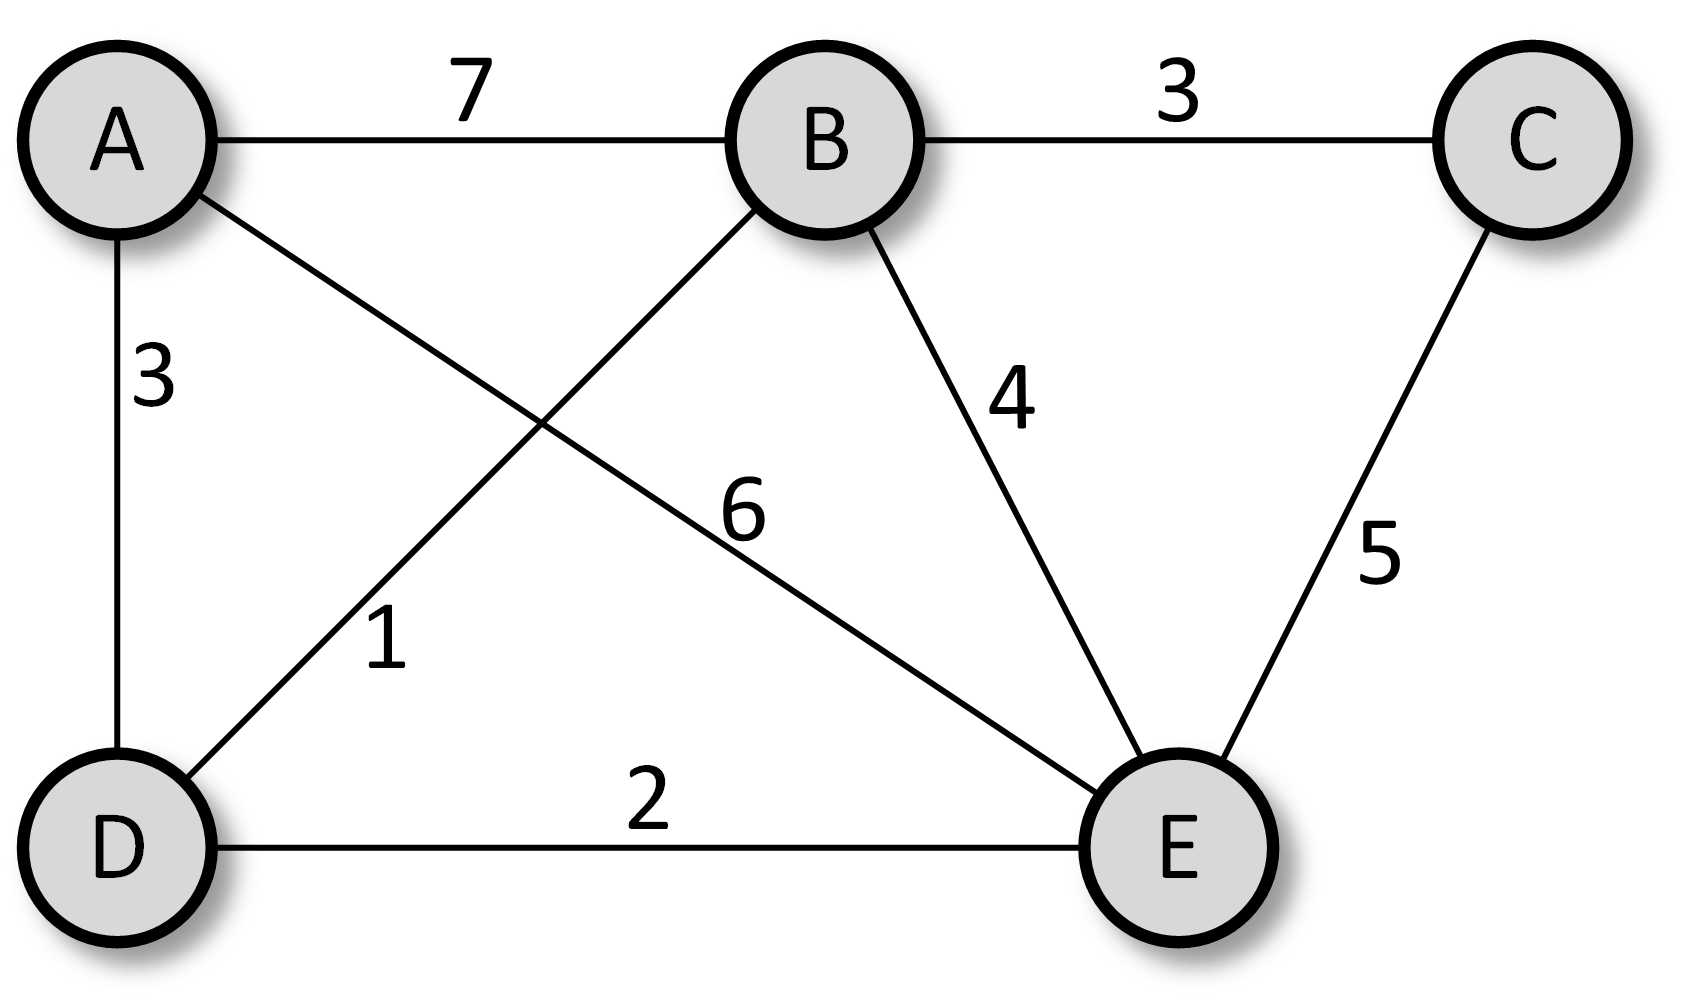
\includegraphics{graphs2.eps}
\caption{\label{fig:graphs2}Graph for problems 3}
\end{figure}
\end{problem}

\begin{problem}{4}
Explain how the Bellman-Ford algorithm can be modified to find
the shortest--paths to a destination node from all other nodes in
the graph.
\end{problem}

\begin{thebibliography}{1}

\bibitem{ref:Bert}Bertsekas, D. and Gallager, R.: ''\emph{Data
Networks}'', 2nd edition, 1992

\bibitem{ref:Algo}Cormen, T. H., Leiserson, C. E. and Rivest, R.
L.: ''\emph{Introduction to Algorithms}'', 1990

\end{thebibliography}

\end{document}
